%%%%%%%%%%%%%%%%%%%%%%%%%%%%%%%%%%%%%%%%%%%%%%%%%%%%%%%%%%
\frame {\frametitle{What is a server?}
%%%%%%%%%%%%%%%%%%%%%%%%%%%%%%%%%%%%%%%%%%%%%%%%%%%%%%%%%%
\begin{itemize}
    \item Servers are computers that provide ``services'' to ``clients''
	\begin{itemize}
		\item Typically designed for reliability and to service a large number of requests
		\item Dual-socket servers are the fundamental building block of cloud infrastructure
	\end{itemize}
	\item Organizations typically require many physical servers to provide various services 
	\begin{itemize}	
		\item Web server, database server, mail server, ...
	\end{itemize}	
	\item Server hardware is becoming more compact
	\begin{itemize}
		\item conserving floor space
		\item improving manageability
		\item power and cooling
	\end{itemize}
\end{itemize}
}


%%%%%%%%%%%%%%%%%%%%%%%%%%%%%%%%%%%%%%%%%%%%%%%%%%%%%%%%%%
\frame {\frametitle{What is a rack?}
%%%%%%%%%%%%%%%%%%%%%%%%%%%%%%%%%%%%%%%%%%%%%%%%%%%%%%%%%%
\begin{itemize}
    \item Servers are grouped, placed, and organized in racks
	\item Equipment are designed in a modular fashion to fit into rack units (1RU = 4.45cm)
	\item A single rack (6 ft or 180cms) can hold up to 42 1U servers
\end{itemize}

	\begin{figure}[h]
		\centering
		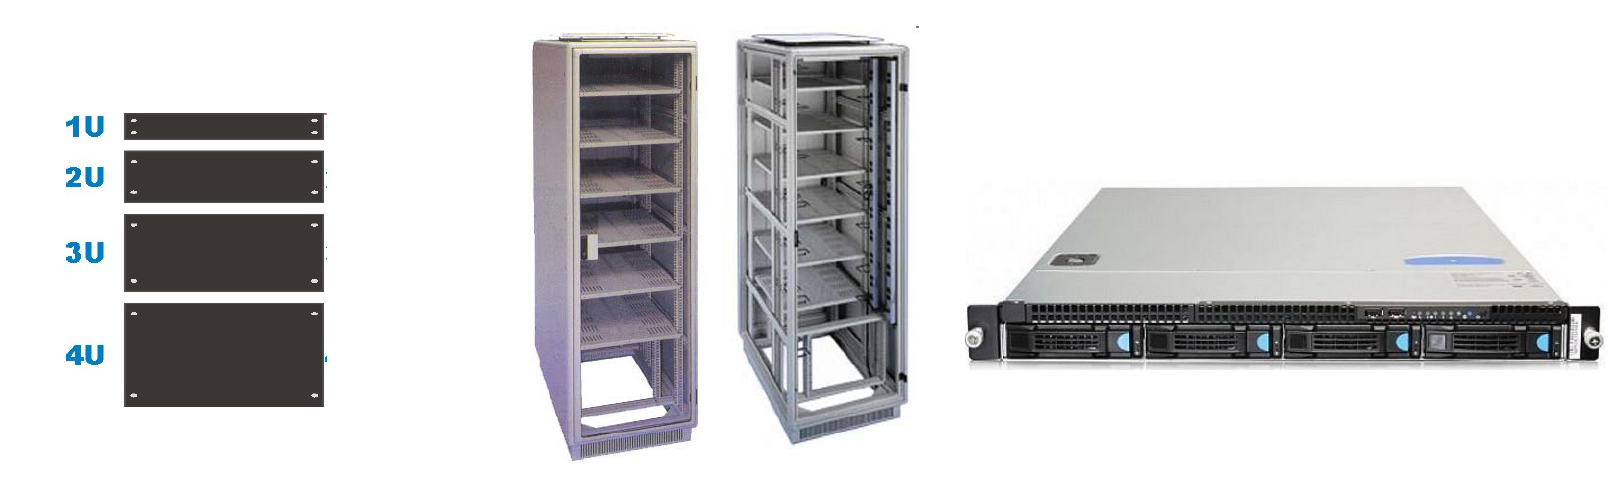
\includegraphics[scale=0.36]{./Figures/server-rack}
		\caption{Global datasphere}
		\label{fig:hdfs}
	\end{figure}

}

%%%%%%%%%%%%%%%%%%%%%%%%%%%%%%%%%%%%%%%%%%%%%%%%%%%%%%%%%%
\frame {\frametitle{What is a data center?}
%%%%%%%%%%%%%%%%%%%%%%%%%%%%%%%%%%%%%%%%%%%%%%%%%%%%%%%%%%
\begin{itemize}
    \item Facility used to house a large number of computer systems and associated components
		\begin{itemize}
			\item Air conditioning
			\item Power supply
			\item Hazard protection
			\item Security and monitoring systems
			\item Networking and connectivity
		\end{itemize}
	\item Let's take a look at a \href{https://www.youtube.com/watch?v=zDAYZU4A3w0}{Google datacenter}
\end{itemize}
}

%%%%%%%%%%%%%%%%%%%%%%%%%%%%%%%%%%%%%%%%%%%%%%%%%%%%%%%%%%
\frame {\frametitle{Problems with privately owned data centers}
%%%%%%%%%%%%%%%%%%%%%%%%%%%%%%%%%%%%%%%%%%%%%%%%%%%%%%%%%%
\begin{itemize}
    \item Expensive to setup (High capital expenses or CAPEX) 
		\begin{itemize}		
		\item Real estate, server and peripherals, ...
		\end{itemize}			
	\item Expensive to operate (High operational expenses or OPEX) 
		\begin{itemize}	
			\item Energy costs (Good data centers have efficiency of 1.7, 0.7 Watts lost for each 1W delivered to the servers)
			\item Administration costs
		\end{itemize}
	\item Difficult for applications to grow/shrink
	\begin{itemize}
		\item How do we map applications to servers?
		\item What if we over/under provision?
	\end{itemize}
	\item Low utilization (30\% server usage considered good)
	\begin{itemize}
		\item Throw money at the performance problem (peak provisioning)
		\item Uneven application fit: each server has CPU, memory, and disk: most applications exhaust one resource, stranding the others
		\item Uncertainty in demand: Demand for a new service can spike quickly
	\end{itemize}
\end{itemize}
}

%%%%%%%%%%%%%%%%%%%%%%%%%%%%%%%%%%%%%%%%%%%%%%%%%%%%%%%%%%
\frame {\frametitle{What if}
%%%%%%%%%%%%%%%%%%%%%%%%%%%%%%%%%%%%%%%%%%%%%%%%%%%%%%%%%%
\begin{itemize}
	\item Turn the servers into a single large resource pool and let services dynamically expand and contract their footprint
as needed?
	\item Two main requirements:
	\begin{itemize}
		\item Means for rapidly and dynamically satisfying application fluctuating resource needs
		\begin{itemize}
			\item Provided by virtualization
		\end{itemize}
		\item Means for servers to quickly and reliably access shared and persistent data
		\begin{itemize}
			\item Provided by programming models and distributed file/storage/database systems
		\end{itemize}		
	\end{itemize}
\end{itemize}
}

%%%%%%%%%%%%%%%%%%%%%%%%%%%%%%%%%%%%%%%%%%%%%%%%%%%%%%%%%%
\frame {\frametitle{What is a cloud then?}
%%%%%%%%%%%%%%%%%%%%%%%%%%%%%%%%%%%%%%%%%%%%%%%%%%%%%%%%%%
\begin{itemize}
	\item Single-site cloud 
	\begin{itemize}
		\item A data center hardware and software that the vendors use to offer the computing resources and services		
	\end{itemize}
	\item Geographically distributed cloud
	\begin{itemize}
		\item Multiple such sites, with each site perhaps having different structure and services
	\end{itemize}
\end{itemize}

	\begin{figure}[h]
		\centering
		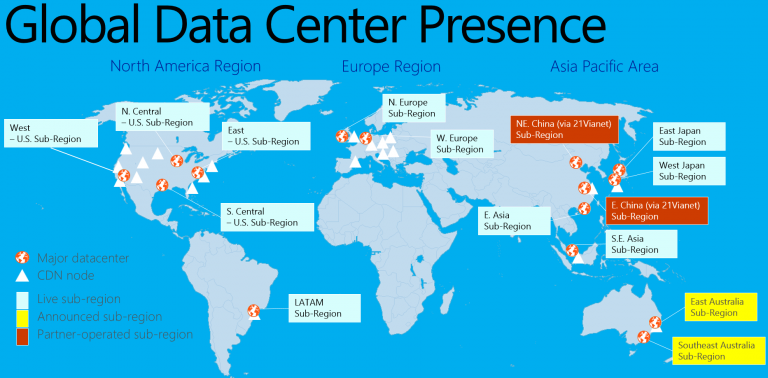
\includegraphics[scale=0.3]{./Figures/azure-regions}
		\caption{Azure: 1 million servers, 100 data centers across 90 countries.}
		\label{fig:hdfs}
	\end{figure}
}

%%%%%%%%%%%%%%%%%%%%%%%%%%%%%%%%%%%%%%%%%%%%%%%%%%%%%%%%%%
\frame {\frametitle{Know the leaders}
%%%%%%%%%%%%%%%%%%%%%%%%%%%%%%%%%%%%%%%%%%%%%%%%%%%%%%%%%%
	\begin{figure}[h]
		\centering
		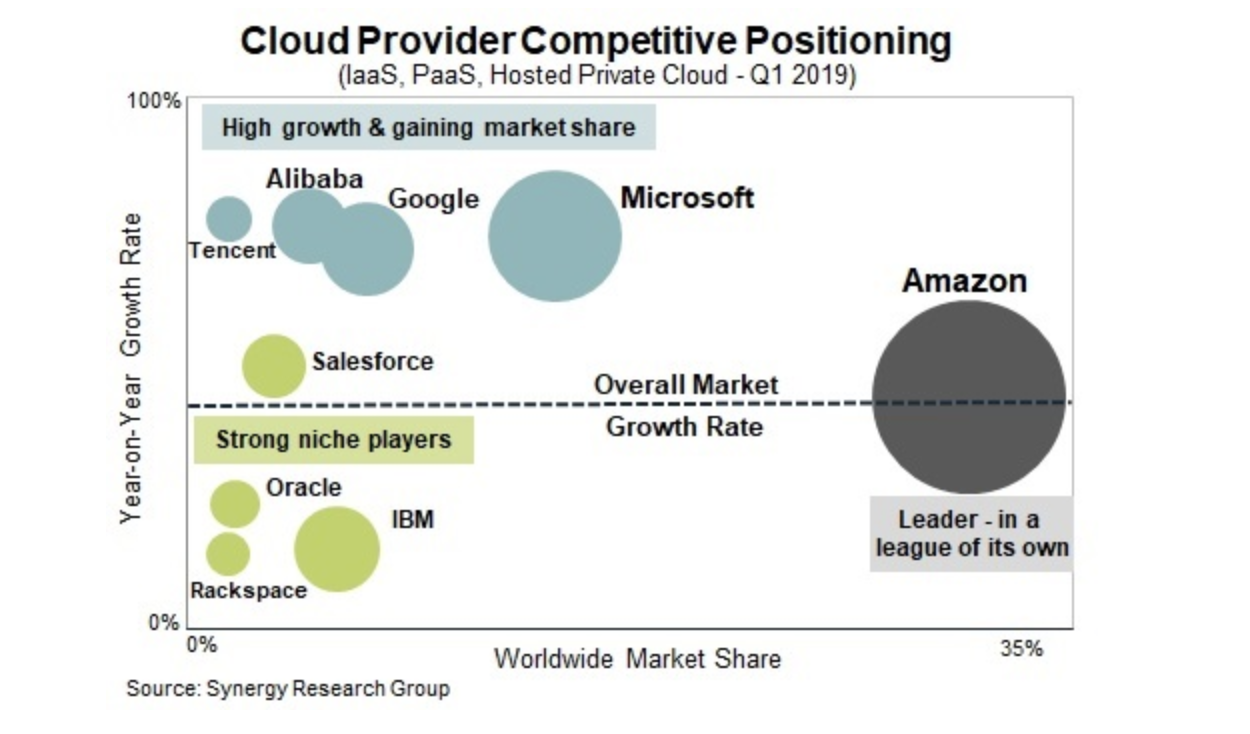
\includegraphics[scale=0.5]{./Figures/cloud-positioning}
		\label{fig:hdfs}
	\end{figure}
}

%%%%%%%%%%%%%%%%%%%%%%%%%%%%%%%%%%%%%%%%%%%%%%%%%%%%%%%%%%
\frame {\frametitle{Cloud Computing}
%%%%%%%%%%%%%%%%%%%%%%%%%%%%%%%%%%%%%%%%%%%%%%%%%%%%%%%%%%

\begin{figure}[h]
	\centering
	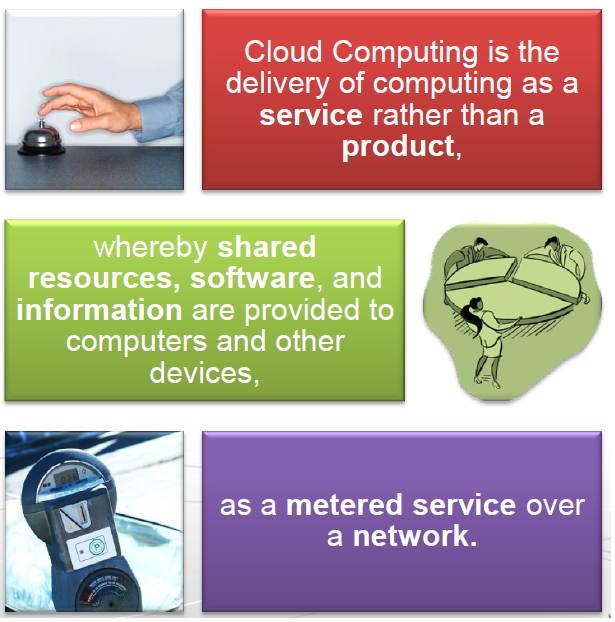
\includegraphics[scale=0.6]{./Figures/cloud-definition}
	\label{fig:hdfs}
\end{figure}
}

%%%%%%%%%%%%%%%%%%%%%%%%%%%%%%%%%%%%%%%%%%%%%%%%%%%%%%%%%%
\frame {\frametitle{IT as a service}
%%%%%%%%%%%%%%%%%%%%%%%%%%%%%%%%%%%%%%%%%%%%%%%%%%%%%%%%%%
\begin{itemize}
	\item How do we offer IT as a service?
	\item Different users have different needs
	\begin{itemize}
		\item Average end user
		\item Mobile app developer
		\item Enterprise systems architect
	\end{itemize}
	\item Let us look at some service models
\end{itemize}
}


%%%%%%%%%%%%%%%%%%%%%%%%%%%%%%%%%%%%%%%%%%%%%%%%%%%%%%%%%%
\frame {\frametitle{Basic cloud service models}
%%%%%%%%%%%%%%%%%%%%%%%%%%%%%%%%%%%%%%%%%%%%%%%%%%%%%%%%%%

\begin{figure}[h]
	\centering
	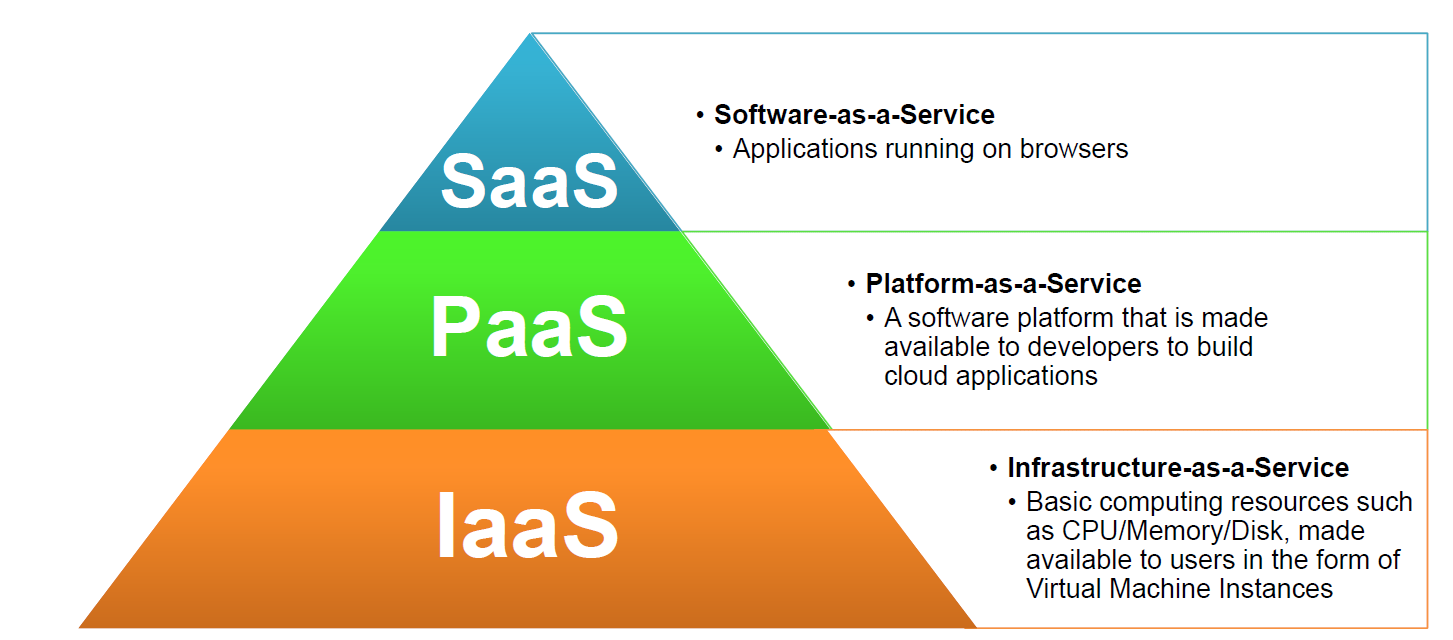
\includegraphics[scale=0.4]{./Figures/cloud-service-models}
	\label{fig:hdfs}
\end{figure}
}

%%%%%%%%%%%%%%%%%%%%%%%%%%%%%%%%%%%%%%%%%%%%%%%%%%%%%%%%%%
\frame {\frametitle{SaaS}
%%%%%%%%%%%%%%%%%%%%%%%%%%%%%%%%%%%%%%%%%%%%%%%%%%%%%%%%%%
\begin{itemize}
	\item Software is delivered as a service over the Internet, eliminating the need to install and run the application on the customer's own computer
	\item Simplifies maintenance and support
	\item You use SaaS products everyday 
	\begin{itemize}
		\item Gmail, Google docs, Youtube, ...
	\end{itemize}
	\item Salesforce.com is a popular commercial pioneer (ERP, CRM, ...)
\end{itemize}
}

%%%%%%%%%%%%%%%%%%%%%%%%%%%%%%%%%%%%%%%%%%%%%%%%%%%%%%%%%%
\frame {\frametitle{PaaS}
%%%%%%%%%%%%%%%%%%%%%%%%%%%%%%%%%%%%%%%%%%%%%%%%%%%%%%%%%%
\begin{itemize}
	\item The Cloud provider exposes a set of tools (a platform) and APIs which allows users to create SaaS applications
	\item The SaaS application runs on the provider's infrastructure
	\item The cloud provider manages the underlying hardware and requirements
	\item Examples: Google App Engine, Windows Azure Web App service
\end{itemize}
}

%%%%%%%%%%%%%%%%%%%%%%%%%%%%%%%%%%%%%%%%%%%%%%%%%%%%%%%%%%
\frame {\frametitle{IaaS}
%%%%%%%%%%%%%%%%%%%%%%%%%%%%%%%%%%%%%%%%%%%%%%%%%%%%%%%%%%
\begin{itemize}
	\item The cloud provider leases to users Virtual Machine Instances (i.e., computer infrastructure) using the virtualization technology
	\item The user has access to a standard Operating System environment and can install and configure all the layers above it
	\item Exampels: AWS EC2, Rackspace, Google Compute Engine
	\item Virtualization is the enabler of IaaS
\end{itemize}

\begin{figure}[h]
	\centering
	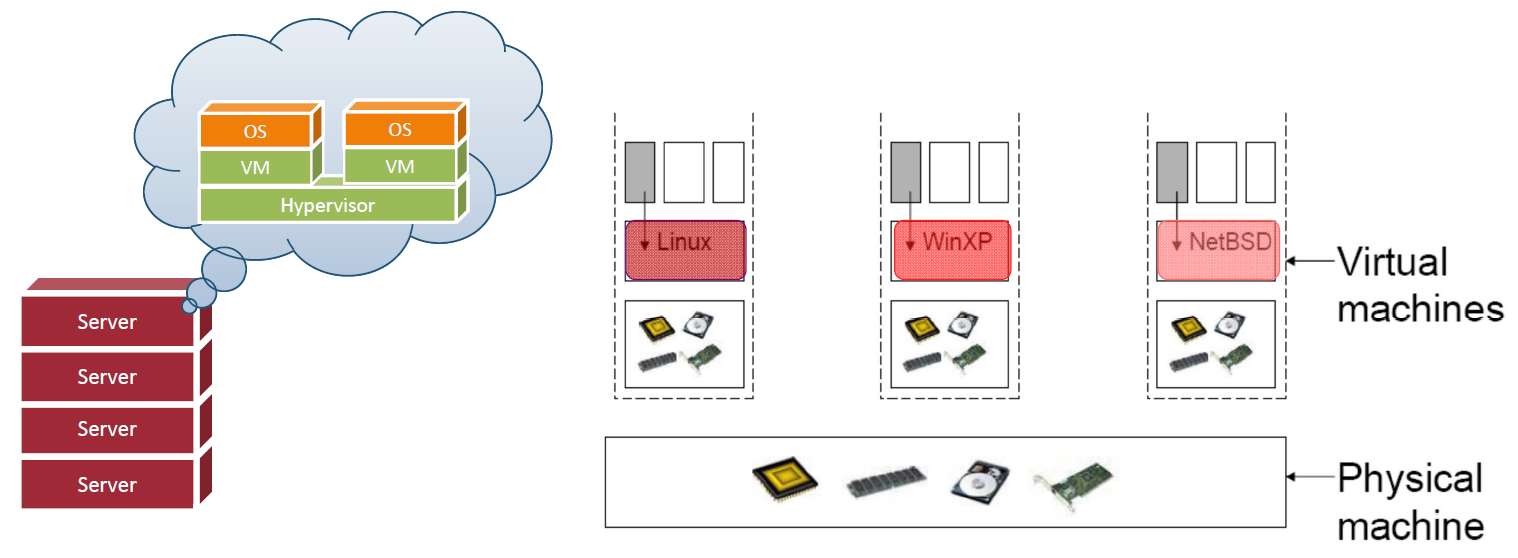
\includegraphics[scale=0.36]{./Figures/virtualization}
	\label{fig:hdfs}
\end{figure}
}

%%%%%%%%%%%%%%%%%%%%%%%%%%%%%%%%%%%%%%%%%%%%%%%%%%%%%%%%%%
\frame {\frametitle{Other services models}
%%%%%%%%%%%%%%%%%%%%%%%%%%%%%%%%%%%%%%%%%%%%%%%%%%%%%%%%%%
\begin{itemize}
	\item Hardware-as-a-service (HaaS)
	\begin{itemize}
		\item You get access to barebones hardware machines, do whatever you want with them, Ex: Your own cluster 
		\item Not always a good idea because of security risks
	\end{itemize}
	\item X-as-a-service, where X can be
	\begin{itemize}
		\item Backend (BaaS), Desktop (DaaS), ...
	\end{itemize}

\end{itemize}
}

%%%%%%%%%%%%%%%%%%%%%%%%%%%%%%%%%%%%%%%%%%%%%%%%%%%%%%%%%%
\frame {\frametitle{The Cloud Stack}
%%%%%%%%%%%%%%%%%%%%%%%%%%%%%%%%%%%%%%%%%%%%%%%%%%%%%%%%%%
\begin{columns}
\column{0.8\linewidth}
	\begin{itemize}
		\item Applications
		\begin{itemize}
			\item Cloud applications can range from Web applications to scientific computational jobs
		\end{itemize}
		
		\item Data
		\begin{itemize}
			\item Old SQL systems (Oracle, SQLServer)
			\item NoSQL systems (MongoDB, Cassandra)
			\item NewSQL systems (TimesTen, Impala, Hekaton)
		\end{itemize}	
		
		\item Runtime environment
		\begin{itemize}
			\item Runtime platforms to support cloud programming models
			\item Example: Hadoop, Spark
		\end{itemize}		
	\end{itemize}
\column{0.2\linewidth}	
	\centering
	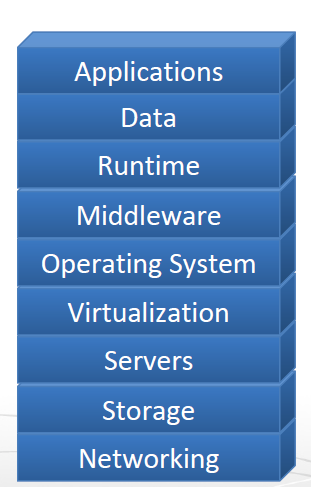
\includegraphics[scale=0.36]{./Figures/cloud-stack}
	\label{fig:hdfs}
\end{columns}
}

%%%%%%%%%%%%%%%%%%%%%%%%%%%%%%%%%%%%%%%%%%%%%%%%%%%%%%%%%%
\frame {\frametitle{The Cloud Stack}
%%%%%%%%%%%%%%%%%%%%%%%%%%%%%%%%%%%%%%%%%%%%%%%%%%%%%%%%%%
\begin{columns}
\column{0.8\linewidth}
	\begin{itemize}
		\item Middleware
		\begin{itemize}
			\item Platforms for Resource Management, Monitoring, Provisioning, Identity Management and Security
		\end{itemize}
		
		\item Operating systems
		\begin{itemize}
			\item Standard Operating Systems used in Personal Computing 
			\item Packaged with libraries and software for quick deployment and provisioning
			\item E.g., Amazon Machine Images (AMI) contain OS as well as required software packages as a ``snapshot'' for instant deployment
		\end{itemize}
		
		\item Virtualization (serverse, storage, networking)
		\begin{itemize}
			\item Key enabler of cloud computing
			\item Providers resource virtualization, multitenancy
			\item Ex: Amazon EC2 is based on the Xen virtualization platform, Azure based on HyperV
		\end{itemize}		
	\end{itemize}
\column{0.2\linewidth}
	\centering
	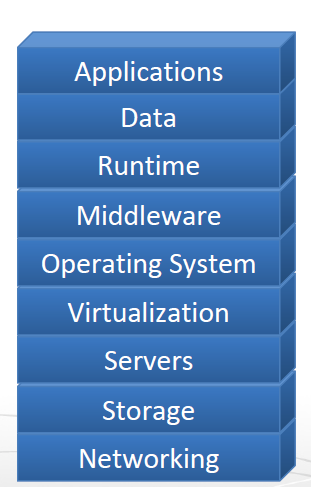
\includegraphics[scale=0.36]{./Figures/cloud-stack}	
\end{columns}
}

%%%%%%%%%%%%%%%%%%%%%%%%%%%%%%%%%%%%%%%%%%%%%%%%%%%%%%%%%%
\frame {\frametitle{Cloud service models and the cloud stack}
%%%%%%%%%%%%%%%%%%%%%%%%%%%%%%%%%%%%%%%%%%%%%%%%%%%%%%%%%%
\begin{figure}[h]
	\centering
	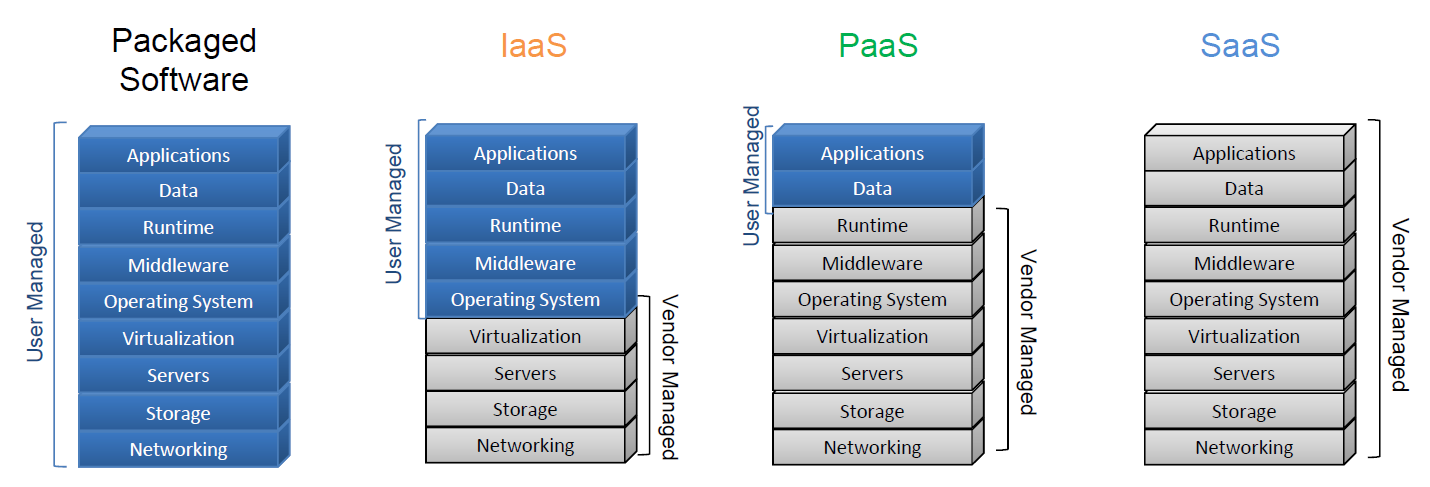
\includegraphics[scale=0.45]{./Figures/cloud-service-cloud-stack}
	\label{fig:hdfs}
\end{figure}
}


%%%%%%%%%%%%%%%%%%%%%%%%%%%%%%%%%%%%%%%%%%%%%%%%%%%%%%%%%%
\frame {\frametitle{Types of clouds}
%%%%%%%%%%%%%%%%%%%%%%%%%%%%%%%%%%%%%%%%%%%%%%%%%%%%%%%%%%
\begin{itemize}
	\item Public (external) cloud
	\begin{itemize}
		\item Open market for on demand computing and IT resources 
		\item Concerns: Limited SLA, reliability, availability, security, and trust
	\end{itemize}

	\item Private (internal) cloud
	\begin{itemize}
		\item For large enterprises with the budget and large-scale IT 
	\end{itemize}

\item Hybrid cloud
	\begin{itemize}
		\item Extend the private cloud(s) by connecting it to other public cloud vendors to make use of their available cloud services
		\item Use the local cloud, and when you need more resources, burst into the public cloud
	\end{itemize}	
\end{itemize}
}


%%%%%%%%%%%%%%%%%%%%%%%%%%%%%%%%%%%%%%%%%%%%%%%%%%%%%%%%%%
\frame {\frametitle{Cloud adoption}
%%%%%%%%%%%%%%%%%%%%%%%%%%%%%%%%%%%%%%%%%%%%%%%%%%%%%%%%%%
\begin{figure}[h]
	\centering
	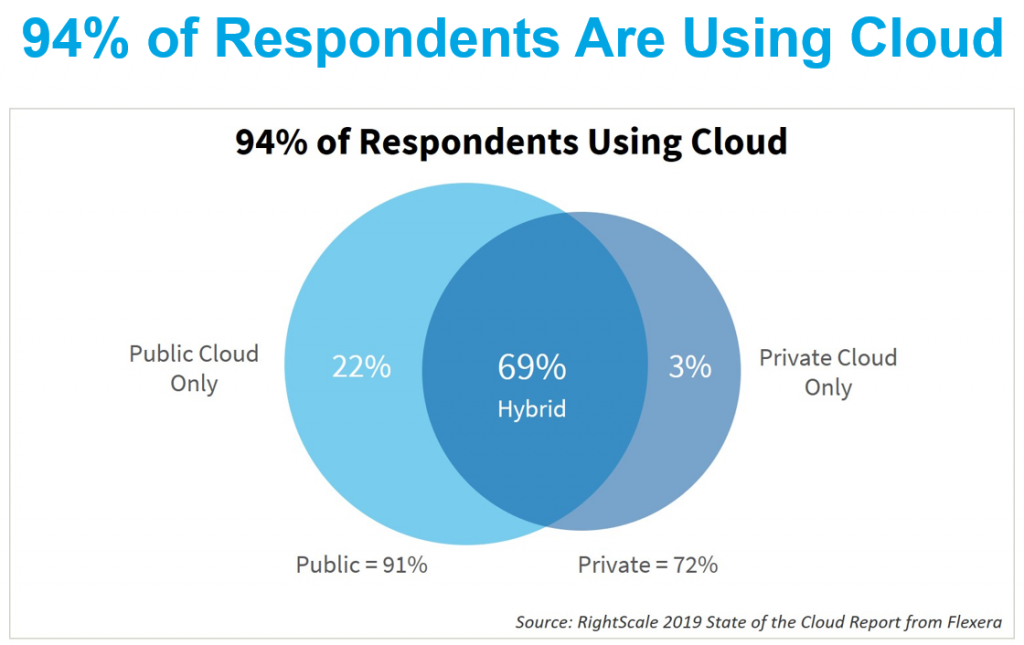
\includegraphics[scale=0.25]{./Figures/cloud-use}
	\label{fig:hdfs}
\end{figure}

\begin{itemize}
\item All major cloud providers are extending their offering to private and hybrid markets
	\begin{itemize}
		\item Example: Google Anthos, Microsoft AzureStack
	\end{itemize}
\end{itemize}
}